%===============================================================================
% $Id: ifacconf.tex 19 2011-10-27 09:32:13Z jpuente $  
% Template for IFAC meeting papers
% Copyright (c) 2007-2008 International Federation of Automatic Control
%===============================================================================
\documentclass[a4paper]{ifacconf}

\usepackage{graphicx,amsmath,url}      % include this line if your document contains figures
\usepackage[round]{natbib}             % required for bibliography
%===============================================================================


% ===============================================================
% Choose the language of the manuscript.
% If in English, choose 
% \def\portugues{0} 
%
% If in Portuguese or Spanish, choose
% \def\portugues{1} 
%
% Note that, if you are writing in Spanish, you need additional 
% adjusts in some parts of the text, which have been put in Portuguese only.
\def\portugues{1} 
% ===============================================================

% If the above line is commented, it is assumed manuscript in English:
\ifx\portugues\undefined
\def\portugues{0}
\fi


\if\portugues0
   \usepackage[english]{babel}
  \else
   \usepackage[spanish,brazil,english]{babel}
\fi

  

\usepackage[T1]{fontenc}
%\usepackage{inputenc}

\usepackage[utf8]{inputenc}

\usepackage{ae}


\if\portugues1
% =====================================================================
% =====================================================================
% If the manuscript is in Spanish, please change the texts adequatelly.
% You may also add other definitions in this part.
 \newtheorem{teorema}[thm]{{\em Teorema}}{ }
 \newtheorem{lema}[thm]{{\em Lema}}{ }
 \newtheorem{corolario}[thm]{{\em Corolário}}{ }
 \newenvironment{prova}{{\bf Prova.}}{ }
% ===============================================================
\fi

\begin{document}


\if\portugues1

   % =====================================================================
   % =====================================================================
   % USE THIS PART IF THE TEXT IS IN PORTUGUES OR SPANISH
   % =====================================================================
   % If the manuscript is in Spanish, please change the texts adequately.
   % =====================================================================
   % 
   \selectlanguage{brazil}

   \begin{frontmatter}

      \title{Controle Digital de Pressão Hidráulica em Módulo de Frenagem para Aplicações ADAS}
      % Title, preferably not more than 10 words.

      %\thanks[footnoteinfo]{Reconhecimento do suporte financeiro deve vir nesta nota de rodapé.}


      \author[First]{Elton Inacio Alves Junior}
      % \author[Second]{Segundo B. Autor} 
      % \author[Third]{Terceiro C. Autor}

      \address[First]{Departamento de Engenharia de Sistemas Eletrônicos, Universidade De São Paulo - USP.}
      % \address[Second]{Faculdade de Engenharia de Controle \& Automação, Universidade do Futuro, RJ (e-mail: autor2@feca.unifutu.rj)}
      % \address[Third]{Electrical Engineering Department, Seoul National University, Seoul, Korea, (e-mail: author3@snu.ac.kr)}


      \selectlanguage{english}
      \renewcommand{\abstractname}{{\bf Abstract:~}}
      \begin{abstract}                % Abstract of not more than 250 words.
         The integration of longitudinal ADAS functions (e.g., ACC/AEB) with the braking system requires a pressure actuator that delivers predictable behavior under physical constraints and model uncertainties of the electro-hydraulic unit. This paper presents a modeling and digital control methodology for wheel brake pressure regulation using an ABS/ESC hydraulic modulator operating in active braking mode, where the pressure reference is treated as an external command generated by a higher-level controller. The plant is described by a lumped nonlinear two-pressure hydraulic model (supply and wheel-channel pressures) with pump and orifice-based flow laws. A local linearization around a braking operating point yields a state-space model that is discretized via ZOH and used to design a discrete-time LQI controller with integral action, combined with a discrete Luenberger observer. Actuator saturations and a discrete valve logic with hysteresis are included to reflect typical modulator operation. Validation is carried out in MATLAB/Simulink through stepwise pressure tracking tests, performance metrics, and a parametric sensitivity sweep to assess robustness. Simulation evidence indicates the feasibility of pressure tracking with command signals consistent with actuation limits, and it provides a reproducible workflow that supports future embedded implementation.

         \vskip 1mm% não altere esse espaçamento
         \selectlanguage{brazil}
         {\noindent \bf Resumo}:  A integração de funções ADAS de controle longitudinal (por exemplo, ACC/AEB) com o sistema de freio demanda um atuador de pressão capaz de responder com previsibilidade, mesmo sob restrições físicas e incertezas do sistema eletro-hidráulico. Este artigo apresenta uma metodologia de modelagem e controle digital para o regulador de pressão por roda em um módulo ABS/ESC operando em frenagem ativa, tratando a referência de pressão como um sinal proveniente de um controlador de nível superior. A planta é representada por um modelo hidráulico não linear concentrado em duas pressões (suprimento e canal de roda), com leis de vazão baseadas em bomba e orifício. A partir de uma linearização local em regime de frenagem, obtém-se um modelo em espaço de estados discretizado por ZOH para síntese de um controlador LQI em tempo discreto, acoplado a um observador discreto de Luenberger, com saturações e lógica discreta de válvulas (com histerese) compatíveis com a atuação típica do modulador. A validação é conduzida em MATLAB/Simulink, com ensaios de seguimento de referência em patamares, análise por métricas de desempenho e varredura de sensibilidade paramétrica para caracterizar robustez. Os resultados em simulação indicam viabilidade do seguimento de pressão com coerência de comandos frente às limitações de atuação, além de oferecerem um fluxo reprodutível para futura migração a execução embarcada.
      \end{abstract}

      \selectlanguage{english}


      \begin{keyword}
         active braking; digital control; hydraulic pressure regulation; LQI; Luenberger observer; ADAS; MATLAB/Simulink.

         \vskip 1mm% não altere esse espaçamento
         \selectlanguage{brazil}
         {\noindent\it Palavras-chaves:} frenagem ativa; controle digital; regulação de pressão hidráulica; LQI; observador de Luenberger; ADAS; MATLAB/Simulink.
      \end{keyword}


      \selectlanguage{brazil}


   \end{frontmatter}
\else
   % ===============================================================
   % ===============================================================
   % USE THIS PART IF THE TEXT IS IN ENGLISH
   % ===============================================================
   % ===============================================================
   % 

   \begin{frontmatter}

      \title{Style for SBA Conferences \& Symposia: Use Title Case for
         Paper Title\thanksref{footnoteinfo}}
      % Title, preferably not more than 10 words.

      \thanks[footnoteinfo]{Sponsor and financial support acknowledgment
         goes here. Paper titles should be written in uppercase and lowercase
         letters, not all uppercase.}

      \author[First]{First A. Author}
      \author[Second]{Second B. Author, Jr.}
      \author[Third]{Third C. Author}


      \address[First]{Faculdade de Engenharia Elétrica, Universidade do Triângulo, MG, (e-mail: autor1@faceg@univt.br).}
      \address[Second]{Faculdade de Engenharia de Controle \& Automação, Universidade do Futuro, RJ (e-mail: autor2@feca.unifutu.rj)}
      \address[Third]{Electrical Engineering Department,
         Seoul National University, Seoul, Korea, (e-mail: author3@snu.ac.kr)}

      \renewcommand{\abstractname}{{\bf Abstract:~}}

      \begin{abstract}                % Abstract of not more than 250 words.
         These instructions give you guidelines for preparing papers for IFAC
         technical meetings. Please use this document as a template to prepare
         your manuscript. For submission guidelines, follow instructions on
         paper submission system as well as the event website.
      \end{abstract}

      \begin{keyword}
         Five to ten keywords, preferably chosen from the IFAC keyword list.
      \end{keyword}

   \end{frontmatter}
\fi

%===============================================================================
%===============================================================================
%===============================================================================


\section{Introdução}

A frenagem automotiva permanece no centro das discussões sobre segurança veicular porque concentra, em um mesmo momento, decisões humanas, limitações físicas do pneu--pista e restrições do sistema atuador. Além de desacelerar o veículo até a parada, o sistema de freio precisa operar com previsibilidade em diferentes condições de carga, aderência e temperatura, preservando dirigibilidade e estabilidade \cite{Rudolf2011,Konrad2014}. Esse requisito torna-se ainda mais explícito quando a demanda de frenagem deixa de ser exclusivamente comandada pelo condutor e passa a ser executada por funções de assistência à condução.

Sistemas Avançados de Assistência ao Condutor (ADAS) utilizam sensores e algoritmos para apoiar o controle longitudinal e lateral do veículo, o que inclui funções como Controle de Cruzeiro Adaptativo (ACC) e Frenagem Autônoma de Emergência (AEB) \cite{Lentin2022}. Nesses casos, a cadeia de controle tende a ser hierárquica: um módulo de alto nível opera uma desaceleração desejada (ou uma demanda equivalente de torque/força) e, a jusante, o sistema de frenagem deve converter essa solicitação em pressão hidráulica efetiva nas rodas. A qualidade dessa conversão não é um detalhe de implementação; ela influencia diretamente o conforto, a repetibilidade e a robustez do comportamento longitudinal, especialmente quando o veículo opera próximo a limites de atuação ou quando há incertezas e ruídos de medição.

Nas arquiteturas atuais, o conjunto eletro-hidráulico associado às unidades ABS/ESC (bomba, válvulas e eletrônica) pode atuar não apenas como modulador durante eventos de escorregamento, mas também como fonte/atuador de pressão em cenários de frenagem ativa. Do ponto de vista de modelagem e projeto de controle, isso traz um desafio concreto: a dinâmica hidráulica é intrinsecamente não linear, dependente de diferenças de pressão e de restrições de vazão, e a atuação é limitada por saturações físicas e pela natureza discreta de válvulas solenóides (tipicamente operando em estados aberto/fechado ou por PWM). Trabalhos recentes exploram tanto modelos concentrados e aplicações experimentais em unidades hidráulicas \cite{HouhuaJing2022,ZengYangHuang2023} quanto estratégias de coordenação e modulação de pressão \cite{Lv2014,ChenLv2017,PressureCoordinatedControl2023}. Ainda assim, ao observar uma implementação embarcada realista, permanece a necessidade de um fluxo de projeto que conecte, de forma rastreável, (i) um modelo hidráulico suficientemente simples para síntese, (ii) um regulador digital em tempo discreto, e (iii) um conjunto explícito de restrições de atuação e hipóteses de operação compatíveis com o uso do módulo ABS/ESC como atuador de frenagem ativa.

Este artigo aborda esse recorte: controle digital de pressão hidráulica por roda (baixo nível), com referência proveniente de um controlador longitudinal de nível superior. A contribuição não é propor um novo paradigma de controle para frenagem, mas consolidar um encadeamento metodológico reproduzível, adequado à transição de \textit{model-in-the-loop} para etapas futuras de implementação embarcada e validação em bancada, alinhado a práticas de verificação orientadas por simulação em sistemas de controle embarcados \cite{KapinskiJamesDeshmukh2016}.

O objetivo do trabalho é projetar e avaliar, em simulação, uma estratégia de seguimento de referência de pressão por roda utilizando o módulo hidráulico (ABS/ESC) como atuador, considerando não linearidades hidráulicas e limitações físicas de atuação. Para isso, emprega-se um modelo hidráulico não linear concentrado em duas pressões (suprimento e canal de roda), linearização local em torno de um ponto de operação de frenagem e síntese de um controlador discreto em espaço de estados do tipo LQI, acoplado a um observador de Luenberger em tempo discreto. As restrições de atuação (saturações) e a lógica discreta de válvulas são incorporadas para manter coerência com o funcionamento esperado do modulador. A validação é conduzida em MATLAB/Simulink, com ensaios de seguimento de referência e análise de sensibilidade paramétrica, de modo a organizar a discussão em termos de desempenho e esforço de atuação, sem extrapolar para conclusões experimentais fora do escopo simulado.

As próximas etapas do artigo estão organizados da seguinte forma: a Seção~\ref{sec:modelagem} descreve o modelo hidráulico e as hipóteses de atuação; a Seção~\ref{sec:controle}  apresenta a linearização, discretização e o projeto do regulador LQI e do observador; a Seção~\ref{sec:simulacao} discute os cenários de simulação e os critérios de avaliação; por fim, a Seção~\ref{sec:resultados} sintetiza as conclusões e aponta continuidades naturais, incluindo a implementação embarcada e a validação em bancada.

\section{Modelagem do atuador eletro-hidráulico e hipóteses de atuação}
\label{sec:modelagem}
Esta seção descreve a planta considerada no artigo e apresenta as hipóteses adotadas para que o problema de controle seja bem delimitado. O recorte assume o módulo eletro-hidráulico associado a unidades ABS/ESC como \textbf{atuador de pressão} em frenagem ativa, isto é, capaz de gerar e modular pressão no canal de roda a partir de comandos elétricos de bomba e válvulas. A descrição física e funcional desses módulos pode ser encontrada em referências clássicas de sistemas de freio e assistência ao condutor \cite{Konrad2014,Rudolf2011} e em trabalhos recentes voltados a controle/validação de unidades hidráulicas \cite{HouhuaJing2022,ZengYangHuang2023}.

\subsection{Da desaceleração à referência de pressão (sinal externo ao regulador)}
Para integrar o regulador de pressão com uma função longitudinal de nível superior (por exemplo, ACC/AEB), é natural que o controlador superior forneça uma demanda em termos de desaceleração desejada. Como este artigo não tem por objetivo validar um modelo completo de veículo, pneu e sistema de freio, adota-se um mapeamento agregador simples para gerar referências de pressão com ordem de grandeza compatível com os ensaios. Assim, a referência por roda é tratada como entrada do problema de controle e pode ser definida por:
\begin{equation}
   P_{\mathrm{ref}}(t) = \frac{m}{A_c}\,\max\big(-a_{\mathrm{ego}}(t),\,0\big),
   \label{eq:aref_to_pref}
\end{equation}
em que $m$ representa a massa equivalente do veículo e $A_c$ agrega, em um único ganho, efeitos de repartição, conversão pressão--força e eficiência do conjunto de freio. O uso desse mapeamento tem um propósito metodológico: \textbf{isolar a dinâmica do atuador hidráulico} sob controle e discutir desempenho e restrições sem confundir o resultado com a qualidade de um modelo longitudinal completo \cite{Lentin2022}.

\subsection{Modelo hidráulico não linear concentrado (duas pressões)}
A planta é modelada por uma representação concentrada em duas regiões compressíveis: a pressão de suprimento/manifold $P_{sup}$ e a pressão no canal de roda $P_w$, em linha com abordagens comuns na literatura para projeto e validação \cite{HouhuaJing2022,Lv2014,ZengYangHuang2023}. O vetor de estados e o vetor de comandos são definidos como:
\begin{equation}
   x(t)=\begin{bmatrix} P_{sup}(t) \\ P_w(t) \end{bmatrix},
   \qquad
   u(t)=\begin{bmatrix} \omega_p(t) \\ u_{in}(t) \\ u_{out}(t) \end{bmatrix},
   \label{eq:states_inputs}
\end{equation}
em que $\omega_p$ é a velocidade da bomba e $u_{in}$ e $u_{out}$ representam os comandos associados às válvulas de entrada e saída (com interpretação on/off ou PWM médio, a depender da leitura).

A dinâmica de pressão decorre da continuidade para fluido compressível:
\begin{equation}
   \dot{P}_{sup} = \frac{\beta}{V_{sup}}\big(Q_{pump}-Q_{in}-Q_{\mathrm{leak},sup}\big),
   \label{eq:pressure_sup}
\end{equation}

\begin{equation}
   \dot{P}_{w} = \frac{\beta}{V_{w}}\big(Q_{in}-Q_{out}-Q_{\mathrm{leak},w}\big),
   \label{eq:pressure_wheel}
\end{equation}
onde $\beta$ é o módulo volumétrico efetivo e $V_{sup}$ e $V_w$ são volumes equivalentes.

A vazão da bomba é modelada por relação afim com $\omega_p$ e termo de vazamento interno (para o retorno), conforme modelos frequentemente adotados em estudos eletro-hidráulicos \cite{MotorParametricDesign2023,WangBingbing2015}:
\begin{equation}
   Q_{pump} = K_b\,\omega_p - K_{lb}\big(P_{sup}-P_{ret}\big).
   \label{eq:qpump}
\end{equation}

As vazões nas válvulas são descritas por lei de orifício (Torricelli/Bernoulli), com coeficiente de descarga, adotando o operador $(\cdot)_+=\max(\cdot,0)$ para impedir raiz de argumento negativo:
\begin{equation}
   Q_{in} = C_{d,in}\,A_{in}(u_{in})\sqrt{\frac{2\big(P_{sup}-P_w\big)_+}{\rho}},
   \label{eq:qin}
\end{equation}
\begin{equation}
   Q_{out} = C_{d,out}\,A_{out}(u_{out})\sqrt{\frac{2\big(P_{w}-P_{ret}\big)_+}{\rho}},
   \label{eq:qout}
\end{equation}
com $A_{in}(u_{in})=A_{in,\max}u_{in}$ e $A_{out}(u_{out})=A_{out,\max}u_{out}$, e $u_{in},u_{out}\in[0,1]$ \cite{ChenLv2017,ProportionalPressureABS2023,Lv2014}. Vazamentos internos podem ser representados por termos proporcionais ao diferencial de pressão, como aproximação de primeira ordem.

As pressões são apresentadas como pressão manométrica (\textit{gauge}) em bar:
\begin{equation}
   P_{g}(t) = \frac{P(t)-P_{ret}}{10^5}\ \text{[bar]}.
   \label{eq:pressao_gauge_bar}
\end{equation}

A Tabela~\ref{tab:parametros_hidraulico_realista} resume o conjunto nominal de parâmetros adotado nos ensaios (caso \textit{realista}), compatível com faixas de pressão de suprimento reportadas para unidades ABS/ESC em frenagem ativa (8--13~MPa) \cite{ZengYangHuang2023,HouhuaJing2022}. Adota-se o limite manométrico
\begin{equation}
   P_{sup,\max}-P_{ret} = 13~\text{MPa}\ (130~\text{bar}),
   \label{eq:psup_max_assumido}
\end{equation}
e a saturação de velocidade da bomba $\omega_{p,\max}$ é parametrizada de modo consistente com esse teto de pressão e o modelo de bomba \eqref{eq:qpump}.

\begin{table}
   \caption{Par\^ametros nominais do modelo hidr\'aulico 2P (caso \textit{realista}).}
   \label{tab:parametros_hidraulico_realista}
   \begin{center}
      \begin{tabular}{l l l}
         \hline
         Par\^ametro                        & S\'imbolo         & Valor (unidade)                       \\
         \hline
         Densidade do fluido                & $\rho$            & $850$ (kg/m$^3$)                      \\
         M\'odulo volum\'etrico efetivo     & $\beta$           & $1{,}5\times 10^9$ (Pa)               \\
         Press\~ao de retorno               & $P_{ret}$         & $1{,}0\times 10^5$ (Pa)               \\
         Volume equivalente (suprimento)    & $V_{sup}$         & $6{,}0\times 10^{-5}$ (m$^3$)         \\
         Volume equivalente (canal/roda)    & $V_{w}$           & $1{,}0\times 10^{-5}$ (m$^3$)         \\
         Coef. descarga (orif\'icio)        & $C_d$             & $0{,}62$ (--)                         \\
         \'Area m\'ax. v\'alvula de entrada & $A_{in,\max}$     & $3{,}0\times 10^{-7}$ (m$^2$)         \\
         \'Area m\'ax. v\'alvula de sa\'ida & $A_{out,\max}$    & $3{,}0\times 10^{-7}$ (m$^2$)         \\
         Vazamento interno da bomba         & $K_{lb}$          & $6{,}8\times 10^{-13}$ ((m$^3$/s)/Pa) \\
         Limite de bomba (ensaio)           & $\omega_{p,\max}$ & $131$ (rad/s)                         \\
         \hline
      \end{tabular}
   \end{center}
\end{table}

\subsection{Hipóteses de atuação e restrições}
O foco é o seguimento de referência de $P_w$ sob restrições físicas típicas do atuador: limites de $\omega_p$, de abertura efetiva das válvulas e faixa plausível de pressão. Além disso, por se tratar de um sistema sujeito a ruído de medição e instrumentação limitada, considera-se a estimação de estados como parte da arquitetura de controle, uma vez que torna o controle mais preciso e robusto. Ressalta-se que o artigo não trata do controle de \textit{slip} roda--pista (ABS no sentido estrito), que exigiria a inclusão explícita de dinâmica longitudinal, pneu e lógica supervisória \cite{Konrad2014}.

\section{Projeto do regulador digital em tempo discreto}
\label{sec:controle}
A estratégia de controle proposta combina: (i) um regulador em espaço de estados para a variável contínua $\omega_p$ e (ii) uma lógica discreta para $u_{in}$ e $u_{out}$, de modo a refletir a natureza de atuação do modulador em arquiteturas convencionais. A síntese é feita em tempo discreto para preservar coerência com implementação embarcada \cite{FranklinPowellWorkman1998,Ogata1997}.

\subsection{Linearização local e discretização}
Como a planta \eqref{eq:pressure_sup}--\eqref{eq:qout} é não linear (principalmente pela dependência em $\sqrt{\Delta P}$), adota-se uma linearização local em torno de um ponto de operação de frenagem $(x_0,u_0)$ que satisfaça $P_{sup,0}>P_{w,0}>P_{ret}$ e diferenciais de pressão positivos nas válvulas. A partir disso, obtém-se um modelo linear incremental no formato:
\begin{equation}
   \delta \dot{x}(t)=A\,\delta x(t)+B\,\delta u(t),
   \qquad
   \delta y(t)=C\,\delta x(t),
   \label{eq:lin_ss}
\end{equation}
com $y(t)=P_w(t)$ como variável controlada. Para síntese digital, o modelo é discretizado com retenção de ordem zero (ZOH), resultando em $(A_d,B_d,C_d)$.

\subsection{Controlador LQI e tratamento de saturações}
Para garantir erro estacionário nulo no seguimento de patamares de referência, incorpora-se ação integral sobre o erro $e(k)=P_{\mathrm{ref}}(k)-P_w(k)$, obtendo uma formulação LQI. Em termos conceituais, o regulador resolve um problema de minimização quadrática em tempo discreto e gera a lei de controle:
\begin{equation}
   \omega_p(k) = \mathrm{sat}\big(\omega_{p,\min},\omega_{p,\max},\; -K_x\,\hat{x}(k)-K_i\,x_i(k)\big),
   \label{eq:lqi_control}
\end{equation}
em que $x_i$ é o estado integrador e $\hat{x}$ é o estado estimado. A saturação é explicitada para manter coerência com limites de atuação e evitar comandos inviáveis. Para reduzir risco de \textit{windup} do integrador sob saturação, emprega-se uma estratégia de anti-\textit{windup} compatível com implementação discreta \cite{FranklinPowellWorkman1998,Ogata1997}.

\subsection{Observador discreto de Luenberger}
Como o modelo possui mais estados do que medições diretas, utiliza-se um observador discreto de Luenberger para reconstruir estados necessários à lei de controle:
\begin{equation}
   \hat{x}(k+1)=A_d\hat{x}(k)+B_d u(k)+L\big(y(k)-C_d\hat{x}(k)\big),
   \label{eq:luenberger}
\end{equation}
onde $L$ é escolhido para garantir dinâmica de estimação suficientemente rápida e robusta ao ruído de medição, dentro das limitações do período de amostragem.

\subsection{Lógica discreta para válvulas}
As válvulas são comandadas por uma lógica simples baseada no erro de seguimento, com histerese para evitar comutação excessiva na presença de ruído e discretização:
\begin{itemize}
   \item se $e(k)>\varepsilon$: prioriza-se pressurização ($u_{in}=1$, $u_{out}=0$);
   \item se $e(k)<-\varepsilon$: prioriza-se alívio ($u_{in}=0$, $u_{out}=1$);
   \item se $|e(k)|\le \varepsilon$: aplica-se retenção (\textit{hold}) ($u_{in}=0$, $u_{out}=0$).
\end{itemize}
Esse arranjo busca representar, de modo controlável, os três modos clássicos do canal hidráulico (pressurizar, reter, aliviar) \cite{Konrad2014}, sem assumir válvulas plenamente proporcionais.

\section{Procedimentos de simulação e critérios de avaliação}
\label{sec:simulacao}
A validação é conduzida em ambiente MATLAB/Simulink, separando-se ensaios em malha aberta e em malha fechada. A malha aberta tem caráter de \textbf{verificação de plausibilidade} do modelo: pressurização, retenção e alívio devem produzir transientes coerentes. Em seguida, a malha fechada avalia o seguimento de referência e o esforço de atuação sob saturações, com e sem ruído de medição, quando aplicável.

O ensaio em malha aberta é organizado em três fases consecutivas: (A) \textit{pressurização}, com degrau em $\omega_p$, $u_{in}=1$ e $u_{out}=0$; (B) \textit{retenção}, com $\omega_p=0$ e $u_{in}=u_{out}=0$; e (C) \textit{alívio}, com $\omega_p=0$, $u_{in}=0$ e degrau em $u_{out}$. Essa sequência representa os três modos clássicos do canal hidráulico (pressurizar, reter, aliviar) e permite verificar, antes de fechar a malha, se o modelo responde de forma causal e consistente com a física de vazões por diferencial de pressão \cite{Lv2014,HouhuaJing2022,Konrad2014}.

Para reduzir subjetividade, os resultados são discutidos com apoio de métricas usuais de desempenho, tais como erro RMS, sobressinal, tempos característicos (subida/acomodação), erro estacionário e esforços máximos de controle. Além disso, realiza-se uma varredura de sensibilidade paramétrica em torno do caso nominal, visando observar degradação de desempenho sob variações de parâmetros físicos (por exemplo, volumes equivalentes, módulo volumétrico efetivo e coeficientes associados à bomba e às válvulas), abordagem alinhada ao uso de simulação como etapa de verificação em sistemas de controle embarcados \cite{KapinskiJamesDeshmukh2016}.

\section{Resultados e discussão}
\label{sec:resultados}
Os ensaios em malha aberta. Figura~\ref{fig:ensaio_malha_aberta_integrado_real} confirmam a coerência causal do modelo: na fase de pressurização, a bomba eleva $P_{sup}$ e, quando $P_{sup}>P_w$, estabelece-se vazão positiva na válvula de entrada e aumento de $P_w$; na retenção, com comandos nulos, o comportamento tende a estabilizar; no alívio, a abertura da válvula de saída promove redução de $P_w$ e fluxo para o retorno. Esse resultado é importante porque evita que inconsistências básicas de modelagem dominem a interpretação do controle \cite{HouhuaJing2022,ZengYangHuang2023}.

\begin{figure}
   \begin{center}
      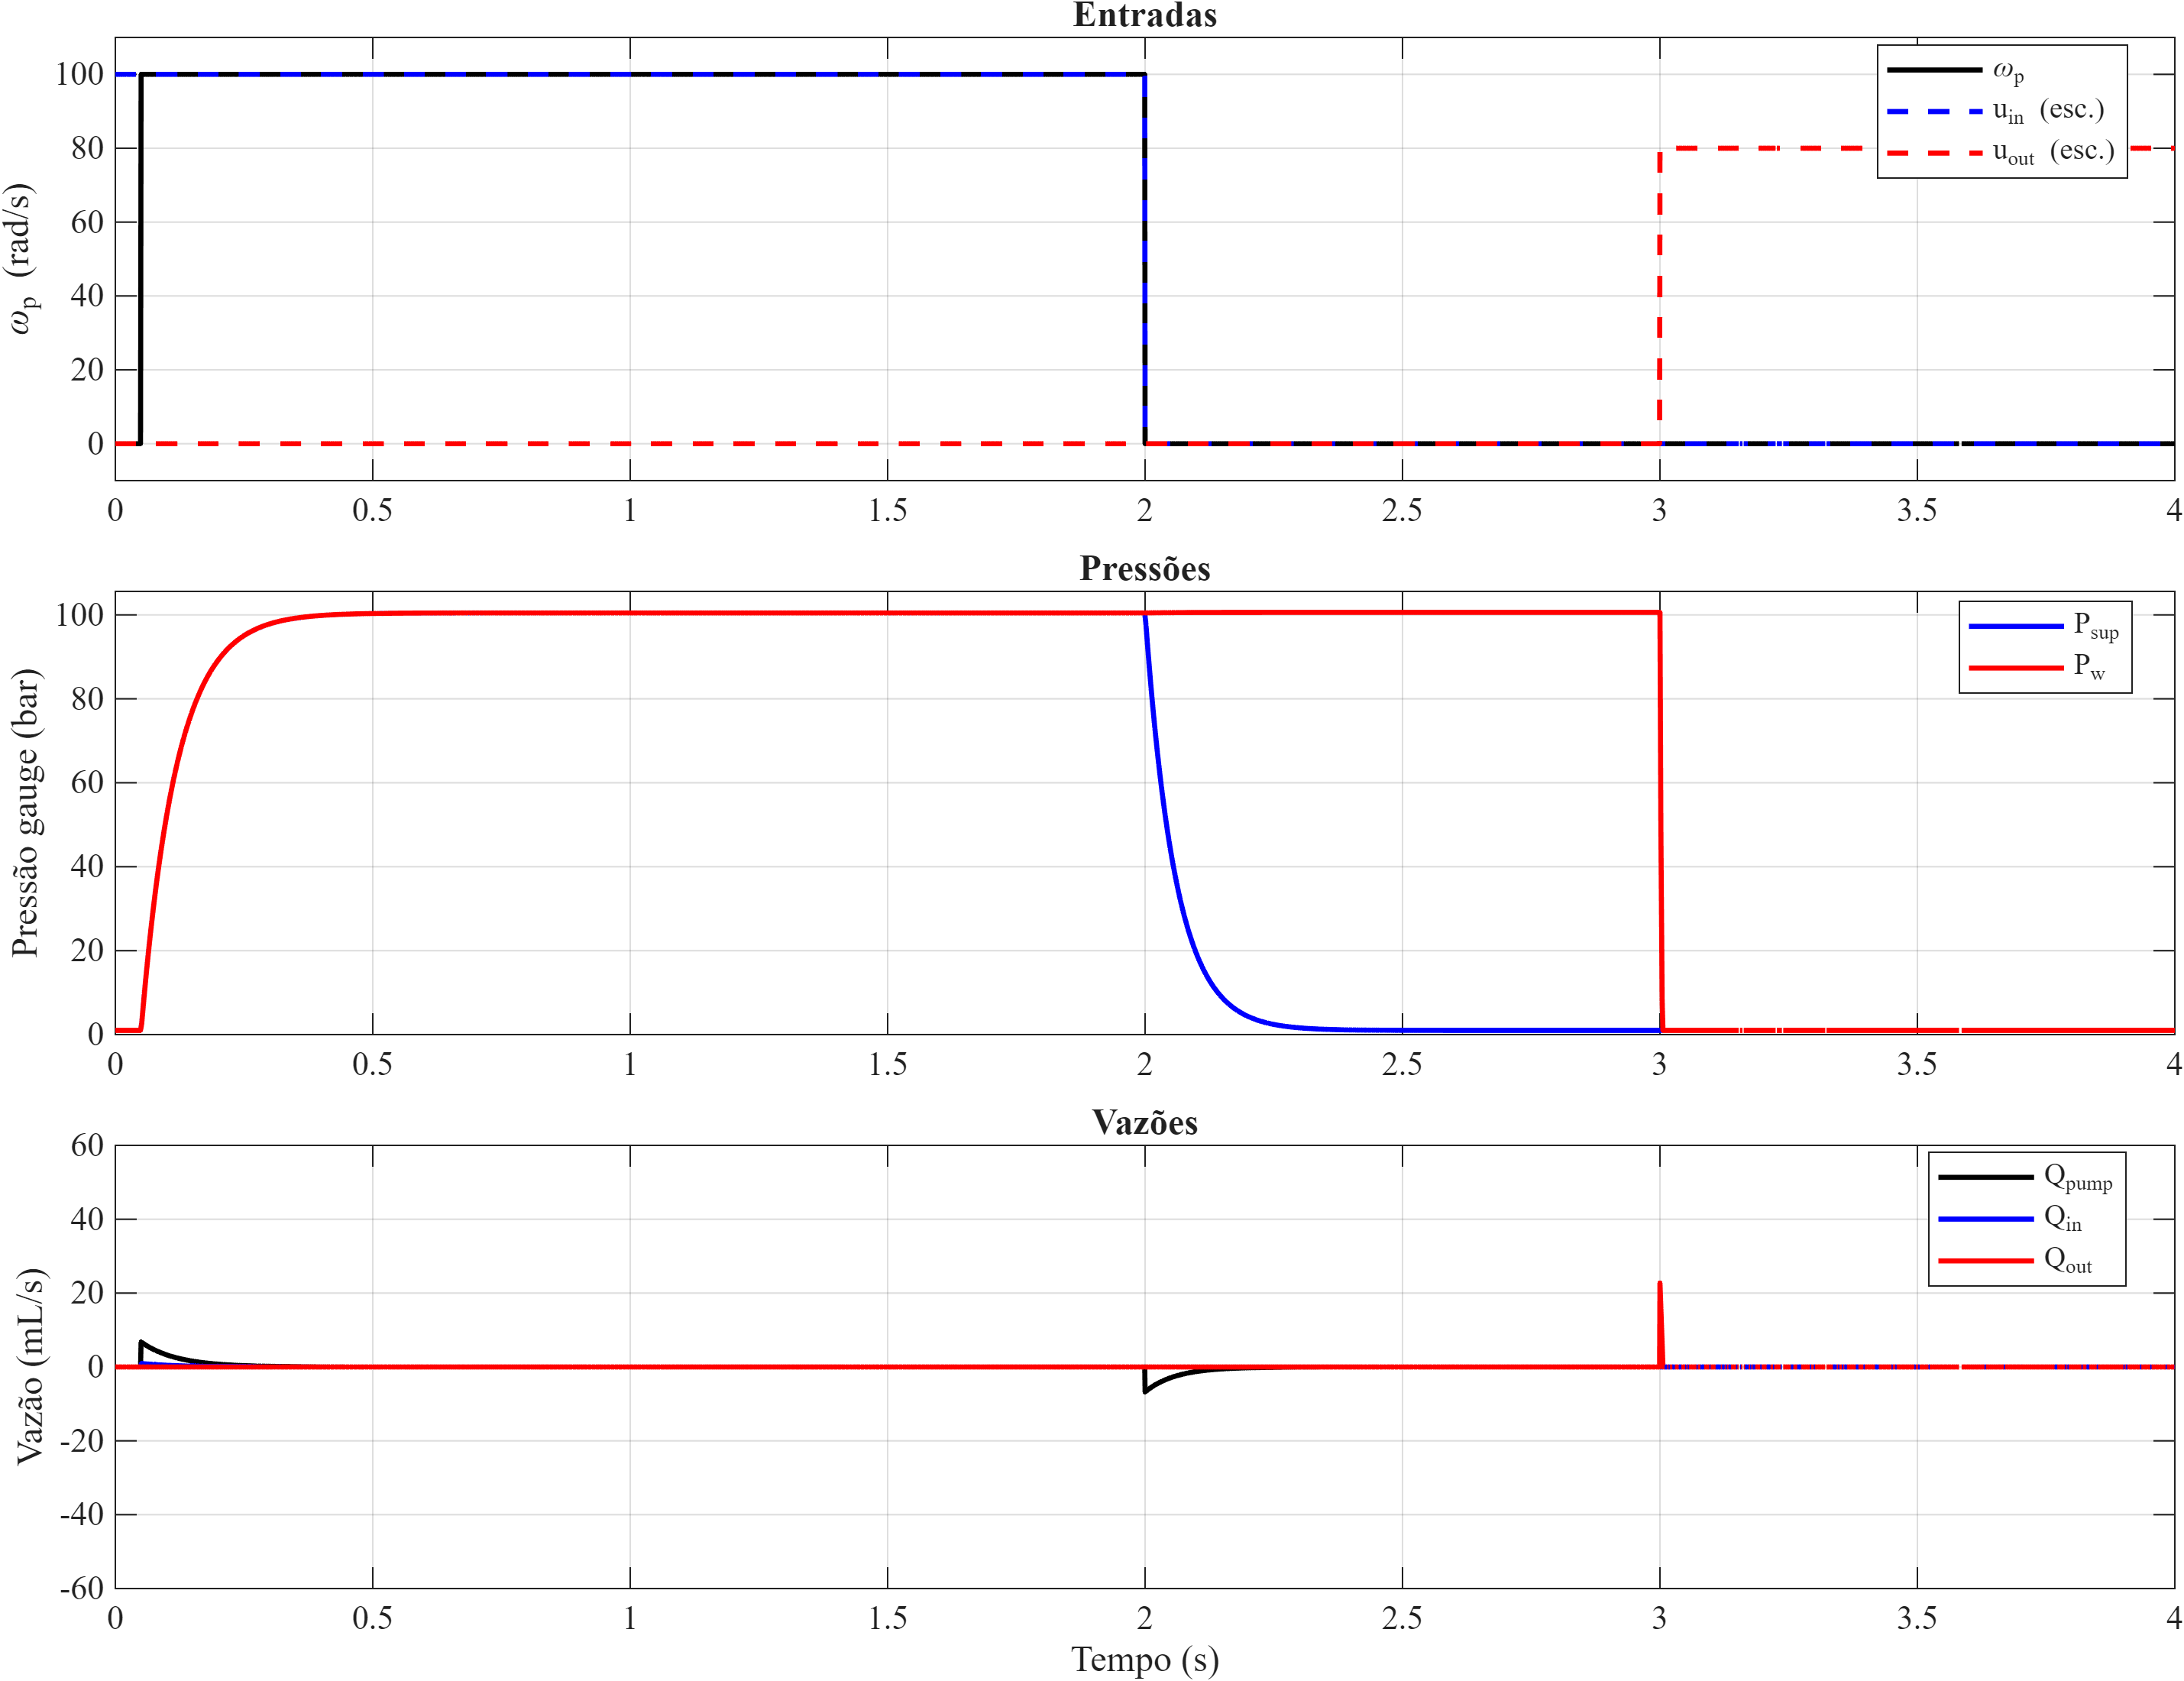
\includegraphics[width=8.4cm]{ensaio_malha_aberta_integrado_real.png}    % The printed column width is 8.4 cm.
      \caption{ensaio malha aberta integrado real.}
      \label{fig:ensaio_malha_aberta_integrado_real}
   \end{center}
\end{figure}

Em malha fechada. Figura~\ref{fig:simulacao_comandos_e_pressao}  a arquitetura LQI+observador demonstra capacidade de rastrear referências em patamares no modelo não linear, com comandos compatíveis com as restrições impostas a $\omega_p$, $u_{in}$ e $u_{out}$. Observa-se que a não linearidade associada às leis de vazão (dependentes de $\Delta P$) tende a produzir assimetrias entre pressurização e alívio, o que reforça a relevância de explicitar saturações e lógica de válvulas no ensaio, em vez de avaliar apenas um modelo linear idealizado \cite{Lv2014,ChenLv2017}. A varredura paramétrica, por sua vez, organiza a discussão de robustez: ao manter ganhos fixos e variar parâmetros, é possível identificar regimes em que o compromisso desempenho--esforço se torna mais crítico e orientar ajustes de pesos do LQI e de limites de atuação.



\begin{figure}
   \begin{center}
      
\includegraphics[width=8.4cm]{simulacao_comandos_e_pressao.png}    % The printed column width is 8.4 cm.
      \caption{simulacao comandos e pressao.}
      \label{fig:simulacao_comandos_e_pressao}
   \end{center}
\end{figure}

\section{Conclusões}
\label{sec:conclusoes}
Este artigo apresentou um fluxo metodológico para projeto e validação, em simulação, de um regulador digital de pressão hidráulica por roda usando o módulo ABS/ESC como atuador em frenagem ativa. A combinação de modelo não linear concentrado, linearização local, síntese LQI em tempo discreto, observador de Luenberger e lógica discreta de válvulas fornece uma arquitetura compatível com restrições de atuação e com requisitos típicos de integração a funções ADAS longitudinais \cite{Lentin2022,Konrad2014}.

Os resultados devem ser interpretados dentro do escopo proposto: evidência em ambiente MATLAB/Simulink, voltada a coerência do controle e à reprodutibilidade do processo de projeto. Como continuidade natural, destacam-se a implementação embarcada do regulador em microcontrolador automotivo, a verificação de temporização do laço de controle e a validação em bancada/HIL com instrumentação mínima de pressão, de modo a consolidar a transferência do \textit{model-in-the-loop} para o ambiente físico \cite{KapinskiJamesDeshmukh2016}.

\bibliography{ifacconf}             % bib file to produce the bibliography
% with bibtex (preferred)

%\begin{thebibliography}{xx}  % you can also add the bibliography by hand

%\bibitem[Able(1956)]{Abl:56}
%B.C. Able.
%\newblock Nucleic acid content of microscope.
%\newblock \emph{Nature}, 135:\penalty0 7--9, 1956.

%\bibitem[Able et~al.(1954)Able, Tagg, and Rush]{AbTaRu:54}
%B.C. Able, R.A. Tagg, and M.~Rush.
%\newblock Enzyme-catalyzed cellular transanimations.
%\newblock In A.F. Round, editor, \emph{Advances in Enzymology}, volume~2, pages
%  125--247. Academic Press, New York, 3rd edition, 1954.

%\bibitem[Keohane(1958)]{Keo:58}
%R.~Keohane.
%\newblock \emph{Power and Interdependence: World Politics in Transitions}.
%\newblock Little, Brown \& Co., Boston, 1958.

%\bibitem[Powers(1985)]{Pow:85}
%T.~Powers.
%\newblock Is there a way out?
%\newblock \emph{Harpers}, pages 35--47, June 1985.

%\bibitem[Soukhanov(1992)]{Heritage:92}
%A.~H. Soukhanov, editor.
%\newblock \emph{{The American Heritage. Dictionary of the American Language}}.
%\newblock Houghton Mifflin Company, 1992.

%\end{thebibliography}

\appendix
% Apêndices foram omitidos para manter o artigo conciso.
\end{document}
